\section{Creating Language in MPS}
\label{sect:LANGDEF}

The proposed \textsc{Ingrid} method accepts grammars in the ANTLR v4 notation~\cite{ref:ANTLRBOOK} as input.
Syntax definition in the form of an ANTLR v4 grammar exists for all widely used programming languages --- it is available at \url{https://github.com/antlr/grammars-v4}.
We did not extend the notation with any custom features.

The process of language construction by \textsc{Ingrid} consists of four phases --- the first is parsing of the input grammar, followed by definition of the essential aspects of the language.

\textsc{Ingrid} is currently able to create (i) a full Structure aspect for each element of the given language, (ii) a very basic Editor, and (iii) a basic TextGen aspect.
Therefore, the resulting MPS language has to be adjusted manually to improve its usability, and the remaining aspects not yet supported by \textsc{Ingrid} must also be defined.

Our approach differs from the existing projects with similar goals (Section~\ref{sect:RELATED}) especially in the level of automation, and it also has much better support for Editor and TextGen.

\subsection{Running Example}

We describe the \textsc{Ingrid} method, and illustrate the main challenges, using a simplified XML language defined in Figure~\ref{fig:SIMPLEXML}.

\begin{figure}[ht]
\vspace{-2mm}
\centering
\begin{alltt}
\small
\antlrparserrule{document}  : \antlrparserrule{prolog}? \antlrparserrule{comment}? \antlrparserrule{element} ;
\antlrparserrule{prolog}    : \antlrliteral{<?xml } \antlrparserrule{attr}* \antlrliteral{?>} ;
\antlrparserrule{comment}   : \antlrliteral{<!--} \antlrlexerrule{TEXT} \antlrliteral{-->} ;
\antlrparserrule{element}   : \antlrliteral{<} \antlrlexerrule{Name} \antlrparserrule{attr}* \antlrliteral{>} \antlrparserrule{content}* \antlrliteral{</} \antlrlexerrule{Name} \antlrliteral{>}
          |  \antlrliteral{<} \antlrlexerrule{Name} \antlrparserrule{attr}* \antlrliteral{/>} ;
\antlrparserrule{attr}      : \antlrlexerrule{Name} \antlrliteral{="} \antlrlexerrule{TEXT} \antlrliteral{"} ;
\antlrparserrule{content}   : \antlrlexerrule{TEXT} | \antlrparserrule{element} | \antlrparserrule{comment} | \antlrlexerrule{CDATA} ;
\antlrlexerrule{Name}      : \antlrlexerrule{NameStCh} \antlrlexerrule{NameChar}* ;
\antlrlexerrule{DIGIT}     : \antlrregex{[0-9]} ;
\antlrlexerrule{NameChar}  : \antlrlexerrule{NameStCh} | \antlrliteral{-} | \antlrliteral{\_} | \antlrliteral{.} | \antlrlexerrule{DIGIT} ;
\antlrlexerrule{NameStCh}  : \antlrregex{[:a-zA-Z]} ;
\antlrlexerrule{TEXT}      : \antlrregex{~[<"]*} ;
\antlrlexerrule{CDATA}     : \antlrliteral{<![CDATA[} \antlrregex{.*?} \antlrliteral{]]>} ;
\end{alltt}
\caption{ANTLR v4 grammar of the SimpleXML language}
\label{fig:SIMPLEXML}
\vspace{-2mm}
\end{figure}

The grammar of SimpleXML contains elements of the kinds that are listed below.
Each color in Figure~\ref{fig:SIMPLEXML} corresponds to one kind, as indicated by the list item headers.
\begin{itemize}
	\item \textbf{ANTLR v4 keywords} are required by the notation.
	\item \antlrparserrule{\textbf{Parser rules}} describe the structure of a language.
	\item \antlrlexerrule{\textbf{Lexer rules}} describe terminal symbols.
		Any of them can be encoded as a string value or a regular expression.
	\item \antlrliteralnoap{\textbf{String literals}} also represent terminal symbols, but by exact match to a string constant.
	\item \antlrregex{\textbf{String tokens}} are described by regular expressions with a special ANTLR v4 regex notation\footnote{https://github.com/antlr/antlr4/blob/master/doc/lexer-rules.md}.
\end{itemize}
Elements on the right side of a rule can be annotated with EBNF operators (\code{?}, \code{+}, \code{*}) that specify the allowed number of occurrences.

\subsection{Phase 1: Parsing Input Grammar}

Parsing of the input ANTLR v4 grammar of a given language is done using an ANTLR parser that was automatically generated from the grammar of the ANTLR v4 notation itself.
The full parse tree, which comes out of the parser, is quite complex and contains information not relevant for \textsc{Ingrid}.
In order to get a simple representation that is easy to process by the later phases and keeps only information necessary for the construction of MPS languages, several steps of post-processing of the parse tree are performed.
An output is a custom AST-like structure that represents the grammar, especially the hierarchy of parser rules, in a way more suitable for MPS.

The representation of lexer rules (tokens) in the full parse tree has to be simplified too.
In the ANTLR notation, lexer rules can be built from alternatives just like the parser rules --- see, for example, the lexer rule \antlrlexerrule{Name} in Figure~\ref{fig:SIMPLEXML}.
Every tree that represents a lexer rule is flattened into the equivalent regular expression.
We describe the flattening algorithm in the full version of this paper~\cite{ref:TRFULL}.

\subsection{Phase 2: Structure}

In the next phase, the complete structure of the MPS language is automatically generated from the AST that represents syntax of the input language.
Elements of the Structure aspect are derived from the AST nodes, and linked appropriately.
Therefore, structure of the MPS language is similar to the original ANTLR grammar.

When designing the procedure for translating AST nodes (i.e., grammar rules) into the MPS language structure, we faced several challenges.
The main challenge is that a grammar typically contains rules that do not directly correspond to programming language constructs.
Such rules exist at the intermediate layers of a syntax hierarchy.
Their purpose is to enable easier understanding and maintenance of the grammar by humans.
Nevertheless, presence of the intermediate layers would significantly complicate usage of the language in MPS, and the layers are actually not necessary for construction of an MPS language.
We show examples illustrating this problem, which we call a \emph{layer problem}, later in this section.
As a part of the \textsc{Ingrid} method, we have designed an approach to eliminate the unnecessary layers --- we call it the \emph{shortcut} approach.
However, before focusing on the intermediate layers, we describe the basic principles of translation from AST into Structure.

In MPS, each concept of the language (i.e., every AST node) is represented by an object that may have a parent, some children, and properties.
Additionally, the object may also contain references to objects representing other AST nodes.
The parent-child relationships between objects that make the Structure aspect are derived from the grammar rules.
If a rule has multiple alternatives, then a distinct object (MPS concept) has to be created for each alternative.
The name of a concept (object) in MPS is composed from (1) the name of the AST node and (2) the number indicating the position of the respective alternative on the right-hand side of the rule.

\begin{figure}[ht]
\vspace{-3mm}
\centering
\begin{alltt}
\small
\mpsstkeyword{concept} Element\_1 \mpsstkeyword{extends} BaseConcept
        \mpsstkeyword{implements} IContent, IElement

  \mpsstkeyword{properties:}
  \mpsstproperty{Name\_1} : Name
  \mpsstproperty{Name\_2} : Name
  
  \mpsstkeyword{children:}
  \mpsstproperty{Attribute\_1} : Attribute[\mpsstcardinality{0..n}]
  \mpsstproperty{Content\_2}   : IContent[\mpsstcardinality{0..n}]
\end{alltt}
\caption{Structure aspect of the \code{Element{\_}1} concept}
\label{fig:ELEMENTSTRUCT}
\vspace{-2mm}
\end{figure}

Consider the parser rule \antlrparserrule{element} from the grammar in Figure~\ref{fig:SIMPLEXML}.
Its first alternative represents the full XML element with content.
Figure~\ref{fig:ELEMENTSTRUCT} shows the relevant fragments of the Structure aspect for the MPS concept (object) named \code{Element{\_}1} that corresponds to the alternative.
The object contains two properties, one for each reference to the lexer rule \antlrlexerrule{Name}.
String literals, such as the opening and closing brackets (\antlrliteral{\textless}, \antlrliteral{/\textgreater}) in XML, are omitted because they will be defined only in the Editor aspect for this concept.

References to other parser rules are captured by pointers to child objects.
The types of child objects, such as \code{IContent} in \code{Element{\_}1}, are determined as follows.
Consider the \antlrparserrule{content} rule from SimpleXML.
An object corresponding to any one of the four alternatives could be the actual value anywhere the \antlrparserrule{content} rule is referenced.

Our solution is to use interface concepts.
For each rule with multiple alternatives on the right side, first an interface concept is defined, and then one object that implements the given interface is created for each alternative.
The resulting fragment of the language structure contains one interface \mpsinterface{IContent} that is implemented by four object concepts \mpsconcept{Content{\_}1}, $\ldots$, \mpsconcept{Content{\_}4}.

Now we can illustrate the layer problem on the behavior of auto-completion in MPS.
Suppose that a user inserted a fresh node of the type \mpsconcept{Element{\_1}}, and would like to insert another XML element inside.
The auto-completion mechanism of MPS offers four options that are displayed in the left part of Figure~\ref{fig:LAYERPROBLEM}.
Each option represents one of the MPS concepts that implement the interface \mpsinterface{IContent}.

\begin{figure*}[ht]
	\centering
	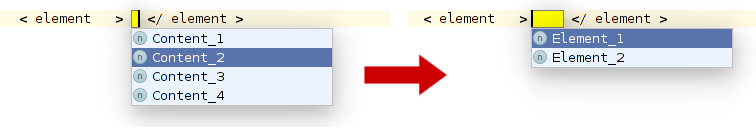
\includegraphics[scale=0.5]{./images/layer_problem.png}
	\caption{Layer problem in auto-completion}
	\label{fig:LAYERPROBLEM}
\end{figure*}

However, in order to correctly insert another nested element, a user has to perform two steps:
\begin{enumerate}
	\item Insert an object (node) of the type \mpsconcept{Content{\_}2} inside the \mpsconcept{Element{\_}1} node. The \mpsconcept{Content{\_}2} object has only a single child node of the interface type \mpsinterface{IElement}.
	\item Then, the user must again trigger auto-complete and insert either an \mpsconcept{Element{\_}1} node or \mpsconcept{Element{\_}2} into the \mpsconcept{Content{\_}2} node. See the right part of Figure~\ref{fig:LAYERPROBLEM}.
\end{enumerate}
The difficulty here is that, in the first step, the user either (i) has to correctly guess what option to select in the auto-complete menu, or (2) to remember the order of alternatives in the grammar rule.

Similarly, if the user would like to replace a nested \mpsconcept{Element{\_}1} node with, for example, a \mpsconcept{Comment} node, then both intermediary layers have to be deleted before she gets back to the original selection among the concepts \mpsconcept{Content{\_}1}, $\ldots$, \mpsconcept{Content{\_}4}.

Intermediary layers have no visual appearance, and therefore it is very difficult for users to see what is actually happening and they may get confused easily.
The layer problem is addressed by the shortcut approach, which we describe in the following paragraphs.

\noindent\textbf{The Shortcut Approach.}
The key idea of this approach is to skip all the intermediary layers (nodes) in the syntax tree, and consider just the nodes to be directly offered to the user through the auto-completion menu.
Specifically, the \antlrparserrule{content} rule from the SimpleXML grammar expands ultimately into the nodes highlighted using the bold font in Figure~\ref{fig:CONTENTEXPAND}.

\begin{figure}[ht]
\small
\textbf{Content{\_}1} (TEXT) \\
\ \ \ Content{\_}2 $\rightarrow$ \textbf{Element{\_}1} \\
\ \ \ Content{\_}2 $\rightarrow$ \textbf{Element{\_}2} \\
\ \ \ Content{\_}3 $\rightarrow$ \textbf{Comment} \\
\ \ \ \textbf{Content{\_}4} (CDATA)
\caption{Leaf nodes of the parser tree fragment that has the \antlrparserrule{content} rule as its root}
\label{fig:CONTENTEXPAND}
\vspace{-2mm}
\end{figure}

For the input that consists of an AST node $N$ and the grammar rule $R$ that expands $N$, the procedure implementing the shortcut approach systematically traverses the full tree (AST) in order to identify each AST node that (i) may appear in some derivation chain starting by the rule $R$ from $N$ and (ii) does not belong to any intermediary layer.
We call them \emph{end nodes}.
Our algorithm that can recognize intermediary layers is described in the full version~\cite{ref:TRFULL}.

We use the name \emph{shortcut approach} for this algorithm, because it creates shortcuts from the given rule to end nodes, by the virtue of hiding all intermediary layers.
The primary use case for shortcuts is to generate options for the auto-completion menus, such that only the end nodes are offered.
Shortcuts have to be considered when nodes are inserted, and also when they are deleted.
In each case, the whole chain including possibly multiple intermediary AST nodes must be added, respectively deleted.

\subsection{Phase 3: Editor}
\label{sect:EDITORDEF}

Having the complete structure of the new MPS language, the next phase is to define the visual representation of all concepts (AST nodes) in the projectional editor.
As we said in Section~\ref{sect:MPS}, MPS uses a cellular system that enables the language developer to arrange the children and properties of an AST node in a table-like manner.
The specific goal of this phase is to create the Editor aspect for each language concept, such that all its attributes --- name, properties, children --- are projected using the respective cell types.

The main problem that we had to address is the absence of information about the code layout and whitespace in ANTLR grammars.
Here we present a solution that is only partially automated.

We observed that the most tedious and error-prone step in the manual definition of the Editor aspect is the creation of cells for all literals (keywords), properties, children, and other fields of a given concept.
This step can be very easily automated.

Our solution that we implemented in the current version of \textsc{Ingrid} is to create all the cells and place them in a single row.
Further adjustments of the layout, such as indentation and line breaks, can be done very efficiently by the user in the MPS IDE.
The resulting layout is illustrated on the example of the \mpsconcept{Element{\_}1} concept in Figure~\ref{fig:EDITORADJUST} (Appendix~\ref{sect:APX}).

Based on our experience, it takes a very short time to manually adjust the layout into a form much better than any fully automated heuristic could achieve.
We actually experimented with several heuristics to derive a useful code layout automatically, but all of them produced rather suboptimal results.

\subsection{Phase 4: Text Generation}
\label{sect:TEXTGENDEF}

The purpose of the last phase of the MPS language construction is to generate the TextGen aspect for each concept.
Figure~\ref{fig:TEXTGENBASIC} shows a fragment of BaseLanguage code that can be used as the TextGen aspect for \mpsconcept{Element{\_}1}.
The code appends all literals, properties, and children of \mpsconcept{Element{\_}1} to the output buffer.

\begin{figure}[ht]
\begin{alltt}
\small
\mpstgkeyword{text gen component for concept} \mpstgtarget{Element{\_}1} \{
  \mpstgparam{(context, buffer, node)->void} \{
    \mpstgaction{append} \{\mpstgliteral{<}\}; \mpstgaction{append} \$\{\mpstgparam{node}.\mpstgnodeprop{\textit{Name}}{\_}\textit{1}\}; \mpstgaction{append} \{\ \};
    \mpstgaction{append} \$list\{\mpstgparam{node}.\mpstgnodeprop{\textit{Attribute}}{\_}\textit{1}\}; \mpstgaction{append} \{\mpstgliteral{>}\};
    \mpstgaction{append} \$list\{\mpstgparam{node}.\mpstgnodeprop{\textit{Content}}{\_}\textit{2}\};
    \mpstgaction{append} \{\mpstgliteral{</}\}; \mpstgaction{append} \$\{\mpstgparam{node}.\mpstgnodeprop{\textit{Name}}{\_}\textit{2}\}; \mpstgaction{append} \{\mpstgliteral{>}\};
  \}
\}
\end{alltt}
\caption{Basic TextGen aspect for the \mpsconcept{Element{\_}1} concept}
\label{fig:TEXTGENBASIC}
\vspace{-4mm}
\end{figure}

Like in the case of a projectional editor, the main challenge associated with TextGen is to produce valid code with a reasonable layout.
An implementation of TextGen must determine properly where to put line breaks, spaces, and indentation.
For example, in the case of the concept representing an XML element, there must be a space between the element's name and the first attribute, while it is not required between the opening bracket \antlrliteral{\textless} and the name.

Our \textsc{Ingrid} method targets mostly text-based languages, for the concepts of which the visual representation in a projectional editor must be almost equivalent to their plain-text representation.
An obvious choice would therefore be to use the same approach for Editor and TextGen.
Nevertheless, since the Editor aspect has to be adjusted manually, we decided to use a different approach for TextGen.
We designed a procedure based on a simple fully automated heuristic that provides acceptable results --- the output is human-readable and close to standard formatting of source code used by popular IDE tools, although minor tweaks are often needed.

The procedure creates the TextGen aspect for a given language concept in two steps.
First, it generates a basic variant that inserts spaces (or line breaks) in between every two tokens of the textual representation of the concept.
In the second step, spaces are eliminated from places where they are not really needed.
The main criterion is whether the generated textual output can be accepted by a parser of the original language (using the ANTLR grammar).
Again, the specific cases are discussed in the full version~\cite{ref:TRFULL}.
We show the complete TextGen aspect for \mpsconcept{Element{\_}1} in the appendix.

\subsection{Remarks about Grammars}
\label{sect:REMARKSGRAMMARS}

During our work on the \textsc{Ingrid} method, we have observed that practical usability of a resulting MPS language depends on the specific manner in which the input ANTLR grammar is defined.

\noindent\textbf{Adjusting grammars.}
In some cases, a small adjustment of the grammar before the run of \textsc{Ingrid} might yield a better and more useful MPS language.
Here we illustrate this on a simple example.

Figure~\ref{fig:XMLATTRIB} shows the definition of an XML attribute, which is taken from the original XML grammar.
The lexer rule \antlrlexerrule{STRING} says that quotes make a part of the attribute's value.
If the MPS language would faithfully match the grammar, the user would have to always input both quotes together with the value in the projectional editor.

\begin{figure}[ht]
\vspace{-2mm}
\begin{alltt}
\small
  \antlrparserrule{attr} : \antlrlexerrule{Name} \antlrliteral{=} \antlrlexerrule{STRING} ;
  \antlrlexerrule{STRING} : \antlrliteral{"} \antlrregex{~["]*} \antlrliteral{"} | \antlrliteral{\textbackslash'} \antlrregex{~[']*} \antlrliteral{\textbackslash'} ;
\end{alltt}
\caption{Definition of an XML attribute}
\label{fig:XMLATTRIB}
\end{figure}

In SimpleXML, we adjusted the grammar in a way that we show in Figure~\ref{fig:XMLADJUST}.
We turned quotes into literals, ensuring that they will only appear in the projectional editor as string constant cells.

\begin{figure}[ht]
\begin{alltt}
\small
  \antlrparserrule{attr} : \antlrlexerrule{Name} \antlrliteral{="} \antlrlexerrule{TEXT1} \antlrliteral{"} | \antlrlexerrule{Name} \antlrliteral{=\textbackslash'} \antlrlexerrule{TEXT2} \antlrliteral{\textbackslash'} ;
  \antlrlexerrule{TEXT1} : \antlrregex{~["]*} ;
  \antlrlexerrule{TEXT2} : \antlrregex{~[']*} ;
\end{alltt}
\caption{Adjusted fragment of the SimpleXML grammar}
\label{fig:XMLADJUST}
\end{figure}

\noindent\textbf{Breaking original grammars and parsers.}
We also want to point out a general problem with grammar adjustments, which all potential users of \textsc{Ingrid} should be aware of.
The original ANTLR grammar for an input language can be easily changed in a way that, at first, seems harmless and valid in MPS, but the parser generated out of the adjusted grammar stops accepting the original language.

This problem has two main causes: (1) low-level implementation details of token matching in the ANTLR parser and (2) usage of ANTLR grammars for a different purpose in our project.
Since, for practical reasons, it is very important that a parser works for programs written according to the original grammar, adjustments have to be performed carefully by the users of \textsc{Ingrid}.

